\documentclass[tikz,border=8pt]{standalone}
\usetikzlibrary{arrows.meta}

\definecolor{r1fill}{HTML}{F1F8FF}
\definecolor{r1stroke}{HTML}{4DD0E1}
\definecolor{memfill}{HTML}{F1F8ED}
\definecolor{memstroke}{HTML}{4DBA46}
\definecolor{valred}{HTML}{F50000}

\begin{document}
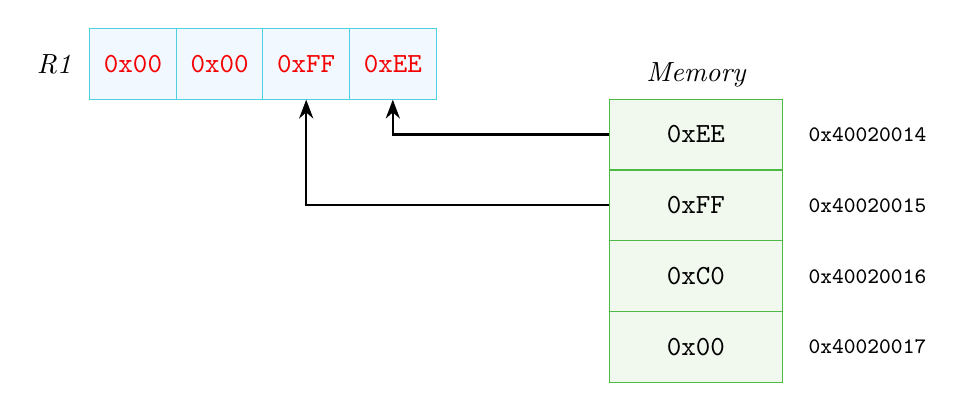
\begin{tikzpicture}[
    x=11mm, y=9mm,
    lbl/.style={font=\itshape},
    addr/.style={font=\footnotesize\ttfamily},
    cell/.style={draw, minimum width=11mm, minimum height=9mm,
                 align=center, font=\ttfamily},
    r1cell/.style={cell, draw=r1stroke, fill=r1fill, text=valred},
    memcell/.style={cell, minimum width=22mm, draw=memstroke, fill=memfill, text=black},
    flow/.style={-{Stealth[length=2.4mm,width=1.8mm]}, thick},
]

% ---- R1 register ------------------------------------------------------------
\node[lbl, anchor=east] at (-0.6,3)  {R1};
\node[r1cell] (b0) at (0,3) {0x00};
\node[r1cell] (b1) at (1,3) {0x00};
\node[r1cell] (b2) at (2,3) {0xFF};
\node[r1cell] (b3) at (3,3) {0xEE};

% ---- Memory column ------------------------------------------------------------
\node[lbl] at (6.5,2.85) {Memory};
\node[memcell] (m0) at (6.5, 2) {0xEE};
\node[memcell] (m1) at (6.5, 1) {0xFF};
\node[memcell] (m2) at (6.5, 0) {0xC0};
\node[memcell] (m3) at (6.5,-1) {0x00};

\node[addr, anchor=west] at ([xshift=2mm]m0.east) {0x40020014};
\node[addr, anchor=west] at ([xshift=2mm]m1.east) {0x40020015};
\node[addr, anchor=west] at ([xshift=2mm]m2.east) {0x40020016};
\node[addr, anchor=west] at ([xshift=2mm]m3.east) {0x40020017};

% ---- Load connectors (memory byte -> R1 byte), only bytes actually read ----
\draw[flow] (m1.west) -| (b2.south);
\draw[flow] (m0.west) -| (b3.south);

\end{tikzpicture}
\end{document}
